% Options for packages loaded elsewhere
\PassOptionsToPackage{unicode}{hyperref}
\PassOptionsToPackage{hyphens}{url}
%
\documentclass[
]{article}
\usepackage{amsmath,amssymb}
\usepackage{iftex}
\ifPDFTeX
  \usepackage[T1]{fontenc}
  \usepackage[utf8]{inputenc}
  \usepackage{textcomp} % provide euro and other symbols
\else % if luatex or xetex
  \usepackage{unicode-math} % this also loads fontspec
  \defaultfontfeatures{Scale=MatchLowercase}
  \defaultfontfeatures[\rmfamily]{Ligatures=TeX,Scale=1}
\fi
\usepackage{lmodern}
\ifPDFTeX\else
  % xetex/luatex font selection
\fi
% Use upquote if available, for straight quotes in verbatim environments
\IfFileExists{upquote.sty}{\usepackage{upquote}}{}
\IfFileExists{microtype.sty}{% use microtype if available
  \usepackage[]{microtype}
  \UseMicrotypeSet[protrusion]{basicmath} % disable protrusion for tt fonts
}{}
\makeatletter
\@ifundefined{KOMAClassName}{% if non-KOMA class
  \IfFileExists{parskip.sty}{%
    \usepackage{parskip}
  }{% else
    \setlength{\parindent}{0pt}
    \setlength{\parskip}{6pt plus 2pt minus 1pt}}
}{% if KOMA class
  \KOMAoptions{parskip=half}}
\makeatother
\usepackage{xcolor}
\usepackage[margin=1in]{geometry}
\usepackage{longtable,booktabs,array}
\usepackage{calc} % for calculating minipage widths
% Correct order of tables after \paragraph or \subparagraph
\usepackage{etoolbox}
\makeatletter
\patchcmd\longtable{\par}{\if@noskipsec\mbox{}\fi\par}{}{}
\makeatother
% Allow footnotes in longtable head/foot
\IfFileExists{footnotehyper.sty}{\usepackage{footnotehyper}}{\usepackage{footnote}}
\makesavenoteenv{longtable}
\usepackage{graphicx}
\makeatletter
\def\maxwidth{\ifdim\Gin@nat@width>\linewidth\linewidth\else\Gin@nat@width\fi}
\def\maxheight{\ifdim\Gin@nat@height>\textheight\textheight\else\Gin@nat@height\fi}
\makeatother
% Scale images if necessary, so that they will not overflow the page
% margins by default, and it is still possible to overwrite the defaults
% using explicit options in \includegraphics[width, height, ...]{}
\setkeys{Gin}{width=\maxwidth,height=\maxheight,keepaspectratio}
% Set default figure placement to htbp
\makeatletter
\def\fps@figure{htbp}
\makeatother
\setlength{\emergencystretch}{3em} % prevent overfull lines
\providecommand{\tightlist}{%
  \setlength{\itemsep}{0pt}\setlength{\parskip}{0pt}}
\setcounter{secnumdepth}{5}
\usepackage{booktabs}
\usepackage{amsthm}
\usepackage{longtable}
\usepackage{comment}

\DeclareMathOperator{\E}{E}
\DeclareMathOperator{\Var}{Var}
\DeclareMathOperator{\Cov}{Cov}
\DeclareMathOperator{\Corr}{Corr}
\DeclareMathOperator{\Tr}{Tr}
\DeclareMathOperator{\PEV}{PEV}

\newcommand{\N}{\mathcal{N}}
\newcommand{\Bern}{\textrm{Bern}}
\newcommand{\Bin}{\textrm{Bin}}
\newcommand{\Beta}{\textrm{Beta}}
\newcommand{\Gam}{\textrm{Gamma}}
\newcommand{\Expo}{\textrm{Expo}}
\newcommand{\Pois}{\textrm{Pois}}
\newcommand{\Unif}{\textrm{Unif}}
\newcommand{\Geom}{\textrm{Geom}}
\newcommand{\NBin}{\textrm{NBin}}
\newcommand{\Hypergeometric}{\textrm{HGeom}}
\newcommand{\HGeom}{\textrm{HGeom}}
\newcommand{\Mult}{\textrm{Mult}}

\newcommand{\matr}[1]{\mathbf{#1}}  % Formatting Matrices
\newcommand{\vect}[1]{\mathbf{#1}}  % Formatting vecotrs
\newcommand{\bfbeta}{{\boldsymbol\beta}}
\newcommand{\bhat}{\hat{\vect{b}}}
\newcommand{\ehat}{\hat{\vect{e}}}
\newcommand{\ghat}{\hat{\vect{g}}}
\newcommand{\uhat}{\hat{\vect{u}}}
\newcommand{\yhat}{\hat{\vect{y}}}
\newcommand{\Vhat}{\hat{\matr{V}}}
\newcommand{\Phat}{\hat{\matr{P}}}
\newcommand{\betahat}{\hat{\bfbeta}}
\newcommand{\thetahat}{\hat{\theta}}
\newcommand{\half}{\frac{1}{2}}
\newcommand{\distr}[1]{{\text{\small{\scshape #1}}}}
\newcommand\independent{\protect\mathpalette{\protect\independenT}{\perp}}
    \def\independenT#1#2{\mathrel{\setbox0\hbox{$#1#2$}%
    \copy0\kern-\wd0\mkern4mu\box0}} 
\usepackage{booktabs}
\usepackage{longtable}
\usepackage{array}
\usepackage{multirow}
\usepackage{wrapfig}
\usepackage{float}
\usepackage{colortbl}
\usepackage{pdflscape}
\usepackage{tabu}
\usepackage{threeparttable}
\usepackage{threeparttablex}
\usepackage[normalem]{ulem}
\usepackage{makecell}
\usepackage{xcolor}
\ifLuaTeX
  \usepackage{selnolig}  % disable illegal ligatures
\fi
\usepackage[]{natbib}
\bibliographystyle{plainnat}
\usepackage{bookmark}
\IfFileExists{xurl.sty}{\usepackage{xurl}}{} % add URL line breaks if available
\urlstyle{same}
\hypersetup{
  pdftitle={Estimation of Breeding Values},
  pdfauthor={Guillaume Ramstein \& Peter Sørensen},
  hidelinks,
  pdfcreator={LaTeX via pandoc}}

\title{Estimation of Breeding Values}
\author{Guillaume Ramstein \& Peter Sørensen}
\date{2025-04-10}

\begin{document}
\maketitle

{
\setcounter{tocdepth}{2}
\tableofcontents
}
\subsection*{Learning objective:}\label{learning-objective}
\addcontentsline{toc}{subsection}{Learning objective:}

This section introduces the basic concepts of breeding value estimation such as:

\begin{itemize}
\tightlist
\item
  basic principle behind estimating breeding values
\item
  accuracy of estimated breeding values
\item
  use of genetic relationships for estimating breeding values
\item
  the connection between genetic parameters and estimated breeding values
\item
  different methods, data sources and experimental designs for estimating breeding values
\end{itemize}

\section{Introduction}\label{introduction}

Breeding value estimation is a fundamental component of breeding programmes, in which the breeding value of each individual is predicted to inform subsequent selection decisions.
The breeding value for an individual is the total additive genetic value which is passed on to the offspring. Thus the breeding value is not a measure of how good an individual is in itself,
but rather of the effect its genes will have in the population. Breeding values are used for:

\begin{itemize}
\tightlist
\item
  comparing individuals in the breeding population and selecting parents for the next generation
\item
  predicting the consequences of selection decisions
\item
  describing genetic differences over time (result of previous selection)
\end{itemize}

The true breeding value (TBV) for an individual cannot be observed. It is only possible to measure its phenotypic value, which is influenced both by genotype and environment. Therefore, we need a way to infer the breeding value from the phenotypic value and select individuals based on an estimated breeding value (EBV). This is the objective of breeding value estimation.

\section{Basic principles for breeding value estimation}\label{basic-principles-for-breeding-value-estimation}

Breeding values are estimated using information on phenotypes and genetic relationships for individuals in a breeding population. As introduced previously the phenotype for a quantitative trait is the sum of both genetic and environmental factors. In general the amount of information provided by the phenotype about the breeding value is determined by the narrow sense heritability (\(h^2\)), which measures the proportion of additive genetic variance contained in the total phenotypic variance. Furthermore phenotypes collected from close relatives provide more information about the breeding value of an individual. In this section we will illustrate these principles using phenotypic data and genetic relationships used for for estimating breeding values. We will now try to derive a general approach for predicting breeding values for any situation. Even though the procedure is general we will use a simple example to describe it.

\subsection{Genetic model}\label{genetic-model}

The breeding value is based on an assumption of a specific genetic model. In general the total genetic effect for an individual is the sum of both additive and non-additive effects that affect the trait:

\begin{align}
    y &=\mu+a+d+i+\epsilon
\end{align}

where \(\mu\) is the population mean, \(a\) is the breeding value (i.e.~additive effect), \(d\) is the dominance effect, \(i\) is the epistasis effect, and \(e\) is the environmental deviation (or residual) not explained by the genetic effects in the model. However, only the additive genetic effects are passed on to the offspring and therefore contributes to the breeding value. In contrast non-additive genetic effects (dominance and epistasis) are degraded by recombination and are not inherited, even though they may be important for the individual's phenotype. Therefore we only consider the additive genetic model as the basis for breeding value estimation:

\begin{align}
            y=\mu+a+e    \notag
\end{align}

The true breeding value for an individual is the sum of all additive genetic effects that affect the quantitative trait:
\begin{align}
        a_{i}=\sum_{k=1}^{K}a_{ik} \notag
\end{align}

where \(a_{i}\) is the total additive genetic effect for the i'th individual, \(a_{ik}\) is the additive genetic effect for loci k, and K is the total number of causal loci. We therefore assume (based on the central limit theory) that the true breeding values, a, and the residual term, \(e\), are normally distributed which means that the observed phenotype is also normally distributed:
\begin{align}
a \sim N(0,\sigma^2_{a}) \notag \\
e \sim N(0,\sigma^2_{e}) \notag \\
y \sim N( \mu,\sigma^2_{a} + \sigma^2_{e}) \notag
\end{align}

\subsection{Expected breeding value conditional on observed phenotype}\label{expected-breeding-value-conditional-on-observed-phenotype}

The breeding value cannot be observed but must be estimated from phenotypic data and genetic relationships between individuals from the breeding population. Estimation of an unknown parameter using statistical modelling expresses the estimated quantity as a mathematical function of the observed data. The question is how this function should look like and what properties the estimated breeding values should fulfill. For breeding purposes one objective for the
estimated breeding values is that the response to selection is maximized.
{[}Henderson, 1963{]} found that the improvement of an offspring generation compared to the parent generation can be maximized when parents are selected
based on the conditional expected value (\(E(a|y)\)) of the true breeding value \(a\)
given the observed phenotypic values \(y\). Under the assumption of multivariate
normality for \(a\) and \(y\) (which are justified under the central limit theorem and the assumptions of many genetic and environmental factors), the expected value of the breeding value conditional on the observed phenotype \(y\) can be written as:
\begin{align}
E(a|y) &= E(a) + Cov(a,y)[Var(y)]^{-1}(y-E(y))
\end{align}
The breeding value is defined as deviation from the general mean which means that the expected value \(E(a)\) of the true breeding value \(a\) is \(E(a)=0\). Therefore the expected value of the breeding value is:
\begin{align}
E(a|y) &= Cov(a,y)[Var(y)]^{-1}(y-\mu)
\end{align}
The expression for the estimate of the breeding value consists of two parts;
The term \(y-E(y)\) shows that the observed phenotypic values are corrected for the
population mean represented by \(\mu\). The term, \(b_{a|y}=Cov(a,y)[Var(y)]^{-1}\), often referred to as the regression coefficient is a weighting factor with which the corrected phenotypic values are multiplied.

To be able to estimate the breeding value we need to determine the values for the terms \(E(a)\), \(E(y)\), \(Var(y)\), and \(Cov(a,y)\) in the expression above. It is possible to derive simple formula's for these terms based on:

\begin{itemize}
\tightlist
\item
  adjusted phenotypic observations for the quantitative trait of related individuals
\item
  heritability of the quantitative trait
\item
  knowledge of inheritance laws and genetic relationships (e.g.~parents, grandparents, siblings) for individuals with phenotypic observations of the quantitative trait
\end{itemize}

This complicated mathematical equation can be expressed as a weighted sum of phenotypic observation for the individual itself and its relatives:

\begin{align}
\hat{a}_i &= w_1(y_1-\hat{\mu})+w_2(y_2-\hat{\mu})+ ...+ w_j(y_j-\hat{\mu})
\end{align}
where \(w_k\) is the weigthing factor for phenotypic observation for individual k. The weight factor depends on the additive genetic variance \(\sigma^2_{a}\), residual variance \(\sigma^2_{e}\) and the additive genetic relationship between individual i and j (explained later).

We will distinguish between true and estimated breeding value using the following notation:
\begin{align}
a &= \text{additive genetic value = true breeding value} \notag \\
\hat{a} &= E(a|y) = \text{estimated additive genetic value = estimated breeding value} \notag
\end{align}

\subsection{Accuracy of breeding value estimates}\label{accuracy-of-breeding-value-estimates}

Estimated breeding values (\(\hat{a}\)) are estimates of the true breeding values (\(a\)), which cannot be observed directly. It is important to determine how well we have estimated the breeding value in relation to the true breeding value. This can be done using accuracy or reliability.

\textbf{Accuracy} is the correlation between the estimated and the true breeding value:
\begin{align}
            r_{a,\hat{a}} &= \frac{\Cov(a,\hat{a})}{\sqrt{\Var(a) \Var(\hat{a})}}
\end{align}

A high correlation means that the estimated breeding value is very accurate.

\textbf{Reliability} is the squared correlation, \(r_{a,\hat{a}}^2\), between the estimated breeding value and the true breeding value. To be able to compute the accuray or reliability of the estimated breeding value we need to determine the values for the terms, \(Cov(a,\hat{a})\), \(Var(\hat{a})\), and \(Var(a)\) in the expression above. It can be shown that the variance of the estimated breeding value is the same as the covariance between the true and estimated breeding value (i.e.~\(Cov(a,\hat{a}) = Var(\hat{a})\)). Therefore the reliability can be expressed as:

\begin{align}
            r_{a,\hat{a}}^2 &= \frac{\Var(\hat{a})}{\Var(a)}
\end{align}

Therefore reliability (\(r_{a,\hat{a}}^2\)) can be interpreted as the part of the genetic variation that is explained by the estimated breeding values whereas the remainder (\(1 - r_{a,\hat{a}}^2\)) is the uncertainty.
Reliability of the breeding value (\(r_{a,\hat{a}}^2\)) is important because it determines how well we can predict an individual's genetic value. It can be used to control the risk of a breeding plan: for example, low \(r_{a,\hat{a}}^2\) leads to greater ``risk'' for both lower and higher true breeding value and we might consider more phenotypic records, in order to make better-informed selection decisions. Lastly reliability is one of the crucial factors that determines the genetic progress (e.g., breeders equation which will be introduced later in the course).

\section{Phenotypic data and genetic relationships are used to estimate breeding values}\label{phenotypic-data-and-genetic-relationships-are-used-to-estimate-breeding-values}

We will illustrate the basic principles of breeding value estimation using some simple examples where the trait has been measured on the individuals themselves or close relatives.

\subsection{Estimation of breeding value and accuracy based on own phenotype:}\label{estimation-of-breeding-value-and-accuracy-based-on-own-phenotype}

An estimate of the breeding value (a) based on own phenotype (y) can be calculated as:
\begin{align}
\hat{a} &= h^2(y-\mu) \notag
\end{align}

Thus the estimated breeding value using own phenotypic record can be computed based on an estimate of the trait heritability (\(h^2\)) and the observed phenotype deviation (\(y-\mu\)). Use of records on the candidate itself is called performance testing. For performance testing to be efficient, the heritability should be at least moderately high (as suggested by equation: \(E(a|y) = h^2(y-\mu)\)).

The accuracy for the breeding value based on own phenotype (\(y\)) can be calculated as:
\begin{align}
            r_{a,\hat{a}} &= \sqrt{h^2} \notag
\end{align}

Estimation of breeding value based on own phenotype is only possible when the trait in question can be measured (directly or indirectly) on the breeding individual, i.e., the candidate to be evaluated for selection. Sometimes this is not possible, e.g., traits that are sex-limited (milk production, female fertility, etc.) cannot be measured in male individuals. Traits like carcass composition and meat quality cannot be measured on live animals, unless an indirect method can be used (e.g.~ultra-sonic measurement of carcass composition). In this situation it might be possible to use phenotypic information on relatives.

\subsection{Estimation of breeding value and accuracy based on phenotypes of close relatives:}\label{estimation-of-breeding-value-and-accuracy-based-on-phenotypes-of-close-relatives}

In practice we often use phenotypic records from close relatives, such as progenies, half-sibs, full-sibs, parents and grandparents. Phenotypes collected on close relatives (as compared to distant relatives) provide more information about the breeding value of an individual (as close relatives share more DNA in common). In the following we will provide a general formula for estimating breeding values and their accuracies using phenotypic information on different types of relatives.

\paragraph*{General formula for estimating breeding values using different sources of information:}\label{general-formula-for-estimating-breeding-values-using-different-sources-of-information}
\addcontentsline{toc}{paragraph}{General formula for estimating breeding values using different sources of information:}

\begin{align}
\hat{a}&=b_{a|y}(y-\mu) 
\end{align}

where the regression coefficient quantifies the weight (or importances) of the phenotypic information:
\begin{align}
b_{a|y}&=\frac{a'nh^2}{(1+(n-1)r} 
\end{align}
where \(a'\) is the genetic relationship between the breeding individual and individuals with phenotypes, \(n\) is the number of phenotypic records, \(h^2\) is the trait heritability, and \(r\) is correlation between individuals with observations (\(r = a^{''}h2\), where \(a^{''}\) = genetic relationship between individuals with records and target). Here we assume that individuals do not share any common environmental component (same litter or same plot).

Thus the importance given to a specific source of information depends on the additive genetic relationship (\(a'\)) with the breeding candidate, the heritability of the trait (\(h^2\)), and the amount of information (\(n\)), i.e.~the number of relatives (progenies or sibs, etc.).

\paragraph*{General formula for reliability of estimated breeding value using different sources of information:}\label{general-formula-for-reliability-of-estimated-breeding-value-using-different-sources-of-information}
\addcontentsline{toc}{paragraph}{General formula for reliability of estimated breeding value using different sources of information:}

\begin{align}
            r_{a,\hat{a}}^2=\frac{(a')^2nh^2}{1+(n-1)r}
\end{align}

Thus reliability depends on the same factors as the estimated breeding value except for the phenotypic value. Although the reliability depends on the number of records it does not depend on the numerical value of phenotypes. From this formula is it clear that higher reliability (and accuracy) can be achived when:

\begin{itemize}
\tightlist
\item
  genetic relationship to individuals with information (a') is high
\item
  there are many records (\(n\) is high)
\item
  heritability (\(h^2\)) is high
\item
  correlation between records (\(r = a''h^2\)) is low (little redundancy in observations)
\end{itemize}

\subsection{Genetic relationship used for estimating breeding value}\label{genetic-relationship-used-for-estimating-breeding-value}

Related individuals share genes and thus resemble each other (have correlated phenotypes, to an extent that depends on additive genetic relationships). Consider a simple parent-offspring example. The offspring get half of the genes from each parent and therefore the breeding value for the offspring is the average of the parents' breeding values plus the Mendelian deviation (the part of the breeding value that is due to random segregation of the genes from each parent):

\begin{align}
        a_{\text{offspring}}=\frac{1}{2}a_{\text{father}}+\frac{1}{2}a_{\text{mother}}+a_{\text{mendelian}} \notag  
\end{align}
(a = additive genetic value = breeding value)

The term \(a_{mendelian}\) is necessary, because two fullsibs \(i\) and \(j\) both having parents \(father\) and \(mother\) receive different random samples of parental alleles. Hence the breeding values \(a_i\) and \(a_j\) of fullsibs \(i\) and \(j\) are not going to be the same. The Mendelian deviation reflects that random contribution of (Mendelian) segregation to breeding values of individuals.

In this equation the \(\frac{1}{2}\) refers to the additive genetic relationship which in this example indicates that the offspring receives half of its genes from its parent. In general the weight given to a specific source of information depends on the additive genetic relationship with the candidate. Examples of different types of additive genetic relationships (\(A_{ij}\)) between the various sources (j) and the individual itself, i.e.~the candidate to be evaluated (i), can be seen in the table below.

\begin{center} 
\begin{tabular}{|c|c|}
  \hline
  Relative  &  $A_{ij}$\\
  \hline
  Self  &  1.0    \\
  \hline
  Unrelated  &  0    \\
  \hline
  Mother  &  0.5 \\
  \hline
  Father  &  0.5 \\
  \hline
  Grandparent  &  0.25 \\
  \hline
  Half-sib  &  0.25 \\
  \hline
  Full-sib  &  0.5 \\
  \hline
  Cousin  &  0.0625 \\
  \hline
  Progeny  &  0.5 \\
  \hline
  Twin(MZ/DZ)  &  1/0.5 \\
  \hline
\end{tabular}
\end{center}

\subsection{Estimation of breeding values using phenotypic information from multiple sources}\label{estimation-of-breeding-values-using-phenotypic-information-from-multiple-sources}

Several factors influence which sources of information to use when estimating
breeding values for a trait: what information is available, the heritability of the
trait, and how and on what individuals the trait can be measured. Therefore in practice it is common to combine information from several sources.
As already mentioned, all information available is usually utilized when an animal's breeding value is predicted. The weight given to a specific source of information depends on the additive genetic relationship with the candidate, the heritability and the amount of information, i.e.~the number of progenies or sibs, etc.

\begin{itemize}
\item
  Phenotypic records on progenies are generally the most accurate source
  of information for genetic evaluation (high genetic relationship \(a'\) and high \(n\)). The average phenotypic value of a progeny group gives the best indication of the additive genetic value (i.e.~the breeding value) of the candidate. The reliability (and accuracy) of breeding value estimates increases with the size of the progeny group. Progeny testing is useful also when the heritability is low. For example, it can be much more accurate than evaluation on own phenotype when the heritability is low (say, 0.1) and the progeny is large (\textasciitilde100-150). The main disadvantage is that it takes resources (time and money) before results on progenies are available. In animal breeding, progeny testing is often used for male animals as they usually get many more progenies than females, especially when artificial insemination is practiced.
\item
  Phenotypic records on the candidate's sibs, half-sibs and full-sibs, are often
  used in addition to other information, or to give supplementary information,
  for example on traits that cannot be measured on the candidate itself. The accuracy of sib testing depends on the number of sibs that have records. Common-environment effects (e.g.~full-
  sibs raised in the same herd) may bias the estimation of breeding values, unless we are able to adjust for them (e.g., by additional fixed effects in linear models).
\item
  Parental information at different generations (parents, grandparents, etc.) is generally available even before the candidate is born, and can provide information very early. However,
  the genes from each locus of the parents are transmitted at random, so information
  based on pedigree alone is not very accurate, but can be valuable
  as additional information. Moreover, the additive genetic relationship, and thus the proportion of common genes between the candidate and the pedigree, is halved for every generation backwards (at least 0.5 for a parent, 0.25 for a grandparent, etc.). Finally, there is redundancy in the information provided by different generations of parents. Fore example, if there are accurate estimate of the parents' breeding values, then there is little to gain in using information on grandparents (actually, if the parents true breeding values are known, there would be no additional gain of information from grandparents).
\end{itemize}

As already mentioned, all information available is usually utilized when an individual's breeding value is predicted. The weight given to a specific source of information depends on the additive genetic relationship with the candidate, the heritability and the amount of information, i.e.~the number of relatives (progenies, sibs, parents, etc.). In the following sections we will show how breeding values can be calculated when different types of phenotypic information (from different types of relatives) are available.

\section{BLUP a general approach for estimation of breeding values}\label{blup-a-general-approach-for-estimation-of-breeding-values}

Breeding value estimation in animal and plant breeding programmes are nowadays based on the BLUP (Best Linear Unbiased Prediction) method. BLUP allows for estimation of breeding values using phenotypic information for individuals from a general pedigree (with arbitrary relationships among them). BLUP is based on linear mixed model methodology, and BLUP estimates of breeding values can be obtained by solving the mixed model equations. The BLUP method also require a genetic relationship matrix and estimates of variance components (e.g., \(\sigma_a^2\) and \(\sigma_e^2\)).

The estimation of breeding values based on multiple sources of information must correct for the redundancy between them (e.g., the redundant information provided by parents and grandparents). Moreover, they need to be adjusted for average effects in the populations, ``fixed effects''. So far we have referred to that fixed effect as the population mean and we have assumed this adjustment \(\mu\) to be known. Indeed, we defined the true breeding value \(a\) and the non-identifiable environmental effects \(e\) as deviations from a common mean, the average effect of all fixed genetic and environmental factors captured by the population mean \(\mu\). But this is only true in a single idealized population where all selection candidates are kept in the same environment in which they deliver their performances at the same time. In practice the phenotypic records often need to be adjusted for systematic (fixed) environmental effects, such as age, parity, litter size, days open, sex, herd, year, season, management, etc. Several of those effects fluctuate very little over time, so accurate estimates of their effect may be obtained from previous (``historical'') sets of data. Effects of factors like herd, year, season, and management fluctuate more, and are therefore best estimated directly from the data to be used in the genetic evaluations.

Compared to the idealized cases described in the previous section, a practical breeding scenario poses two problems: accounting for heterogeneous sources of genetic information (different types of relatives); and adjusting for fixed effects in the breeding population(s) (fixed environmental or genetic effects).

The BLUP solution to these problems was presented by Charles R. Henderson in several publications (e.g.~Henderson 1973a and Henderson 1975). The key idea behind the solution is to estimate the identifiable environmental factors as fixed effects and to predict the breeding values as random effects simultaneously in a linear mixed model. Here, mixed refers to the presence of two types of effects: fixed effects (identifiable effects from environmental or genetic factors) and random effects (non-identifiable effects from segregating genetic factors and fluctuating environmental conditions). The methodology developed by Henderson is called \textbf{BLUP} and the properties of this methodology are directly incorporated into its name:

\begin{itemize}
\tightlist
\item
  \textbf{B} stands for \textbf{best} which means that the correlation between the true (\(a\)) and the predicted breeding value (\(\hat{a}\)) is maximal or the prediction error variance (\(Var(a - \hat{a})\)) is minimal.
\item
  \textbf{L} stands for \textbf{linear} which means the predicted breeding values are linear functions of the observations (\(y\))
\item
  \textbf{U} stands for \textbf{unbiased} which means that the expected values of the predicted breeding values are equal to the true breeding values
\item
  \textbf{P} stands for \textbf{prediction}
\end{itemize}

BLUP approaches are widely used in genetic evaluations, for both traditional predictions of breeding values and also for predicting genomic breeding values. The popularity of BLUP is not only due to the theoretical foundations behind BLUP, but also the efficient algorithms developed by Henderson for computing predicted breeding values, even in very large breeding populations. The theoretical foundations, and the development of efficient algorithms, together with the availability of large computational resources at a very low price, have made BLUP the de-facto standard for breeding value estimation.

\subsection{Linear Mixed Model}\label{mixedlineareffectsmodel}

The linear mixed model contains the observation vector for the trait(s) of interest (\(y\)), the \textbf{fixed effects} that explain systematic differences in \(y\), and the \textbf{random genetic effects} \(a\) and \textbf{random residual effects} \(e\). A matrix formulation of a general model equation is:
\begin{align}
y &= \mu + a + e \notag
\end{align}
where
\begin{align}
y &: \text{is the vector of observed values of the trait,} \notag \\
\mu &: \text{is the population mean (representing the fixed effect),} \notag \\
a &: \text{is a vector of random genetic effects,} \notag \\
e &: \text{is a vector of random residual effects,} \notag
\end{align}
In the statistical model (specified above) the random effects (\(a\) and \(e\)) and the phenotypes (\(y\)) are considered to be random variables which follow a multivariate normal (MVN) distribution. In general terms the expectations of these random variables are:\\
\begin{align}
a \sim MVN(0,G) \notag \\
e \sim MVN(0,R) \notag \\
y \sim MVN(\mu,V) \notag
\end{align}
where \(A\sigma_a^2\), and \(R=I\sigma_e^2\) are square matrices of genetic and residual (co)variances among the individuals, respectively, and \(V=A\sigma_a^2+I\sigma_e^2\) is the overall phenotypic covariance matrix.

\subsection{Estimating the random genetic effects in the linear mixed model}\label{estimating-the-random-genetic-effects-in-the-linear-mixed-model}

The goal of the BLUP analysis is the estimate the random genetic effects, \(a\), in the linear mixed model specified above. This can be done using the BLUP equations shown below. The best linear unbiased prediction (BLUP) of \(\hat{a}\) is:
\begin{equation}
\hat{a} = GV^{-1}(y - \hat{\mu})
\label{eq:hatublup}
\end{equation}
which is similar to the expression shown earlier for the expected value of the breeding value conditional on the observed phenotype \(y\):
\begin{align}
E(a|y) &= Cov(a,y)[Var(y)]^{-1}(y-E(y))
\end{align}
The BLUP equation for the estimate of the breeding value consists of three parts;
The term, \(y - \hat{\mu}\), shows that the observed phenotypic values are corrected for the population mean represented by \(\hat{\mu}\). The covariance between the true breeding values (\(a\)) and phenotypes (\(y\)) is \(Cov(a,y)=G\). The inverse of the phenotypic covariance matrix is \([Var(y)]^{-1}=V^{-1}\).

\subsection{BLUP breeding values are useful for ranking and selection}\label{blup-breeding-values-are-useful-for-ranking-and-selection}

BLUP estimates of breeding values (EBVs), especially from the linear mixed model including all relationships, are useful tools in selection. Selection on BLUP breeding values maximizes the
probability for correct ranking of breeding individuals and selection on BLUP maximizes genetic gain from one generation to another. There are many factors that
contribute to these advantages of BLUP estimates:

\begin{itemize}
\tightlist
\item
  The linear mixed model makes full use of information from all relatives increases accuracy (precision)
\item
  The breeding values are adjusted for systematic environmental effects in an optimal way. This means that individuals can also be compared across herds, age classes, plots etc, assuming the data is connected
\item
  Non-random mating is accounted for
\item
  Several traits can be analyzed simultanously
\item
  Bias due to culling within generation (e.g., between the 1st and 2nd lactations in dairy cattle) and selection (over generations) is accounted for, assuming that also non-selected individuals' data are included in the analysis.
\end{itemize}

It should, however, be noted that the genetic evaluation is based on phenotypic
observations, and that regardless of how great the BLUP procedure may be, it
cannot compensate for bad data. So a good recording system is necessary for a reliable genetic evaluation and subsequent genetic gain. It should also not be forgotten
that BLUP assumes that the genetic parameters used
are the true ones. In practice that means that EBVs will only be accurate if the estimated genetic parameters are close enough to their true value.\\
It should be noted that there is a potential risk for increased inbreeding
when selection is based on information from all relatives.
The probability that several family members are selected jointly is increased,
which may result in increased inbreeding. To avoid this, and to optimize long-term selection response, selection on BLUP breeding values might be combined
with some restriction on average relationship of the selected individuals.
A useful side effect of genetic evaluation by BLUP estimates is that it gives estimates of the
realized genetic trend. This trend can be observed by comparing BLUP breeding values of
individuals from different years.

\begin{comment}

BLUP is based on linear mixed models methodology. A simple linear model contains fixed effects such as _herd_ or _sex_ of an animal or location of a plant and tries to explain the observations as linear functions of such effects. Because the effects considered in a model cannot account for all factors influencing a given set of observations, every model must have a random residual component. If a linear model contains besides any additional random effects (e.g., random genetic effects at the level of families, or locations), then this model is called a __linear mixed effect model__. 


### Numeric Example {#blupnumericexample}
We want to use a concrete numeric example of a small population to explain how breeding values are predicted using the BLUP methodology. The phenotypic observations consist of measurements of the trait __weaning weight__ in beef cattle. Table 1 gives an overview of the dataset.


\begin{longtable}[t]{rrrrr}
\caption{\label{tab:unnamed-chunk-1}Example Data Set for Weaning Weight in Beef Cattle}\\
\toprule
Animal & Sire & Dam & Herd & Weaning Weight\\
\midrule
12 & 1 & 4 & 1 & 2.61\\
13 & 1 & 4 & 1 & 2.31\\
14 & 1 & 5 & 1 & 2.44\\
15 & 1 & 5 & 1 & 2.41\\
16 & 1 & 6 & 2 & 2.51\\
\addlinespace
17 & 1 & 6 & 2 & 2.55\\
18 & 1 & 7 & 2 & 2.14\\
19 & 1 & 7 & 2 & 2.61\\
20 & 2 & 8 & 1 & 2.34\\
21 & 2 & 8 & 1 & 1.99\\
\addlinespace
22 & 2 & 9 & 1 & 3.10\\
23 & 2 & 9 & 1 & 2.81\\
24 & 2 & 10 & 2 & 2.14\\
25 & 2 & 10 & 2 & 2.41\\
26 & 3 & 11 & 2 & 2.54\\
\addlinespace
27 & 3 & 11 & 2 & 3.16\\
\bottomrule
\end{longtable}





#### Fixed Versus Random Effects {#fixedversusrandomeffects}
Unfortunately, there is no unique and generally accepted definition of which effects should be fixed and which should be random. There are generally accepted guidelines of how to classify effects as fixed or random. Certain factors such as herd, sex, breed or feeding regimes can be classified unambiguously as fixed effects. On the other hand, breeding values are always treated as random effects. Breeding values have an expected value (of $0$) and have a certain variance (the additive genetic variance, to be estimated). They must therefore be modeled as random effects and these properties must be integrated into the linear mixed model. Furthermore, each individual has a different realization of a breeding value. Exceptions are mono-clonal twins and clones (e.g., vegetatively reproduced plants like potato or tree species).




Table \\ref{tab:fixedversusrandom} lists a few criteria that might be helpful.

\small


\begin{longtable}[t]{>{\raggedright\arraybackslash}p{22em}>{\raggedright\arraybackslash}p{22em}}
\caption{\label{tab:fixedversusrandom}Classification Factors of Fixed and Random Effects}\\
\toprule
fixed effect & random effects\\
\midrule
classes can be defined exactly & realized value come from an underlying distribution\\
the value of a class does not have an apriori expected value & each realization is unique\\
values are exactly estimable & observations are influenced by the variance of the random effect\\
the expected value of a class effect is of primary interest & main interest is on the variance not on the expected value\\
fixed effects can be corrected for & \\
\bottomrule
\end{longtable}

\normalsize



#### Model Specification {#lmemodelspecification}
In a linear mixed effects model a single observation $y_{ijk}$ is decomposed according to equation \\eqref{eq:linearmixedeffectmodelsingleobservation}

\begin{equation}
y_{ijk} = b_i + a_j + e_{ijk}
\label{eq:linearmixedeffectmodelsingleobservation}
\end{equation}

where $b_i$ is the fixed effect of class i  (specific herd, population, location, etc.)stands for the $i-^{th}$ level of a fixed effect, $a_j$ is the $j-{th}$ realization of the random effect $a$ and $e_{ijk}$  is the residual effect of the $k-^{th}$ observation}.  To include all observations of a data set, it is helpful to represent the model in \\eqref{eq:linearmixedeffectmodelsingleobservation} by a matrix-vector notation. This is shown in equation \\eqref{eq:linearmixedeffectmodelmatrixvector}

\begin{equation}
y = Xb + Za + e
\label{eq:linearmixedeffectmodelmatrixvector}
\end{equation}

\begin{tabular}{llp{10cm}}
where  &  &  \\
       &  $y$      &  vector of length $n$ of all observations \\
       &  $b$      &  vector of length $p$ of all fixed effects  \\
       &  $X$      &  $n \times p$ design matrix linking observations to fixed effects \\
       &  $a$      &  vector of length $n_a$ of random effects \\
       &  $Z$      &  $n \times n_a$ design matrix linking observations to random effects \\
       &  $e$      &  vector of length $n$ of random residual effects.  
\end{tabular}

Furthermore, we assume the following expected values and for the variances. As already mentioned the random effects are defined as deviations and hence their expected value is set to zero. 

\begin{align}
E(a) &= 0 \notag \\
E(e) &= 0 \notag
\end{align}

From this it follows that $E(y) = Xb$. The variance-covariance matrices for the random effects are set to 

\begin{align}
Var(a) &= G \notag \\ 
Var(e) &= R \notag
\end{align}

Under the assumption that $Cov(a,e^T) = 0$, we can compute $Var(y) = Z * Var(a) * Z^T + Var(e) = ZGZ^T + R = V$. 

In model \\eqref{eq:linearmixedeffectmodelmatrixvector} the vectors $b$ and $a$ are unknown. They contain the fixed and random effects which must be estimated (or predicted). The solution of the model \\eqref{eq:linearmixedeffectmodelmatrixvector} for the unknowns $b$ and $a$ leads to estimates $\hat{b}$ for the fixed effects $b$ and for predicted random effects $\hat{a}$. 


## Estimating effects in the linear mixed model
The solutions to the effects $b$ and $a$ in the mixed model presented above are obtained using statistical techniques based on matrix algebra and multivariate normal theory. The details of these derivation are not important. Therefore, we are presenting here directly the results. For $\hat{a}$, the best linear unbiased prediction (BLUP) is:

\begin{equation}
\hat{a} = GZ^TV^{-1}(y - X\hat{b})
\label{eq:hatublup}
\end{equation}

We call $\hat{a}$ the best linear unbiased prediction of $a$ or shorter $\hat{a} = BLUP(a)$. For $\hat{b}$, we insert the generalized least squares estimator (GLS) which corresponds to 

\begin{equation}
\hat{b} = (X^T V^{-1} X)^{-1} X^T V^{-1} y
\label{eq:hatbetahatblue}
\end{equation}

The matrix $(X^T V^{-1} X)^{-1}$ denotes the inverse of the matrix $(X^T V^{-1} X)$.  Analogously to $\hat{a}$, $\hat{b}$ is called the best linear unbiased estimator of the fixed effects $b$. In short, we can state $\hat{b} = BLUE(b)$. 

\end{comment}

\begin{comment}

### Sire Model
The application of the linear mixed effects model from \\eqref{eq:linearmixedeffectmodelmatrixvector} to the numerical example in table \\ref{tab:TableBeefExample}. As random effects $a$ we are taking the father $s$ of each animal $i$ with an observation. As fixed effects $\beta$ we are using the herd effect. When fathers are modeled as random effects, then we call this model a __sire model__. Setting up a sire model for the data in table \\ref{tab:TableBeefExample} looks as follows

\begin{equation}
= 
+ 
+ 
\end{equation}

Besides the equation for the sire model we also have to specify the expected values and the variances of all random components. To be able to distinguish the sire model from the general linear mixed effects model, we usually call the random sire effect $s$ and no longer $a$. The expected values for the random variables were already stated when discussing the general linear mixed effects model in section \\ref{lmemodelspecification}. Hence 

\begin{equation}
E(s) = 0 \qquad \text{and} \qquad E(e) = 0 \qquad \rightarrow \qquad E(y) = X\beta
\label{eq:exvaluerandvarsire}
\end{equation}

For the variances there are a few simplifications that we can use in our sire model. The covariance between the random effects $s$ and $e$ are assumed to be $0$. The covariances among the single residual effects are also assumed to be $0$. Hence, the variance-covariance matrix of the residual effects are $Var(e) = I * \sigma_e^2$. The variance of the sire effects $s$ is 

$$
Var(s) = A_s * \sigma_s^2 = G
$$

where $A_s$ is the additive genetic relationship matrix between the sires. We will be deriving the matrix $A_s$ in a later chapter. Because our sires are not related, we can say that $A_s = I$ and hence

$$
G = I * {\sigma_u^2 \over 4}
$$

Now we are ready to set up the mixed model equations from \\eqref{eq:mixedmodeleq} for the sire model. The computation of the numerical solutions from the mixed model equations will be the topic of an exercise.



### Animal Model {#animalmodel}
The mixed model equations are a universal tool to find BLUPs of random effects and BLUEs of fixed effect simultaneously. On the other hand it is not satisfactory that with the sire model only sires obtain predicted breeding values. All information that is known about the mothers was completely ignored when we specified the sire model. A better approach would be to combine all available information from a given population. This can be done by replacing in the sire model the random sire effects by random animals effects. As a result each animal in the dataset receives a random effect which models its breeding value. This type of model is called an __animal model__. Because the animal model has the breeding values of all animals as random effects, they are often referred to with the variable or the vector $a$^[This is not the same as the genotypic value in a single locus model.] and no longer $s$ as in the sire model. The variance-covariance matrix ($Var(a)$) between all animal effects is proportional to the additive genetic relationship matrix $A$ among all animals. We will see in a later chapter how to compute the matrix $A$.

\end{comment}

\begin{comment}


# Linear Models {#intro-predict-breeding-value}
Because, in the more traditional setting^[That means, at this moment, we are ignoring all recent developments made such as genomic selection.] of livestock breeding, we do not have information about allele frequencies and about genotypic values, we have to predict breeding values. For this prediction we can use different sources of information. Currently, we are assuming that this information is all based on records of phenotypic observations. 


### Model Specification {#basic-model}
Although, the phenotypic observation might originate from different sources, we can use one basic model for all of the breeding value predictions. We have already seen a different form of this model in equation \\eqref{eq:phengenenv} in section \\ref{geno-pheno}.  The original model from equation \\eqref{eq:phengenenv} is modified and extended to the model shown below.

\begin{equation}
y_{ij} = \mu_i + g_i + e_{ij}
\label{eq:breedvalpredbasicmodel}
\end{equation}

\begin{tabular}{llp{9cm}}
where  &  &  \\
       &  $y_{ij}$  &  $j^{th}$ record of animal $i$ \\
       &  $\mu_i$   &  identifiable fixed environmental effect \\
       &  $g_i$     &  sum of all additive ($a$), dominance ($d$) and epistatic effects of the genotype of animal $i$ \\
       &  $e_{ij}$  &  random environmental effect associated to observation $j$ of animal $i$
\end{tabular}

<!-- TODO: Improvement on the following paragraph -->
Livestock species are mostly diploid and hence from a given parent only one allele of a given locus is passed to a gamete which can later be found in the parents offspring. Any interaction effects caused by dominance or epistasis are not preserved from parent to offspring. Only the additive effect of a given allele is passed from parent to offspring. The additive genetic part ($a_i$) of $g_i$ in equation \\eqref{eq:breedvalpredbasicmodel} represents the average genetic effect that animal $i$ receives from its parents. It is therefore called the __breeding value__. Because the additive genetic effect is a function of the alleles passed from the parents to the progeny, it is the only component that can be selected for and is therefore the main component of interest from a livestock breeding perspective. Due to the major interest in the genetic additive component, the terms in the basic model in \\eqref{eq:breedvalpredbasicmodel} are re-arranged as follows.

\begin{equation}
y_{ij} = \mu_i + a_i + e_{ij}^*
\label{eq:breedvalpredmodifiedmodel}
\end{equation}

\begin{tabular}{llp{9cm}}
where  &  &  \\
       &  $y_{ij}$  &  $j^{th}$ record of animal $i$ \\
       &  $\mu_i$   &  identifiable fixed environmental effect \\
       &  $a_i$       &  sum of all additive ($a$) genetic effects of the genotype of animal $i$ \\
       &  $e_{ij}^*$  &  dominance, epistatic and random environmental effects of the $j^{th}$ record of animal $i$
\end{tabular}

The same re-arrangement of terms in the basic model is illustrated by Figure \\ref{fig:basicmodelrearrterm}

\begin{figure}
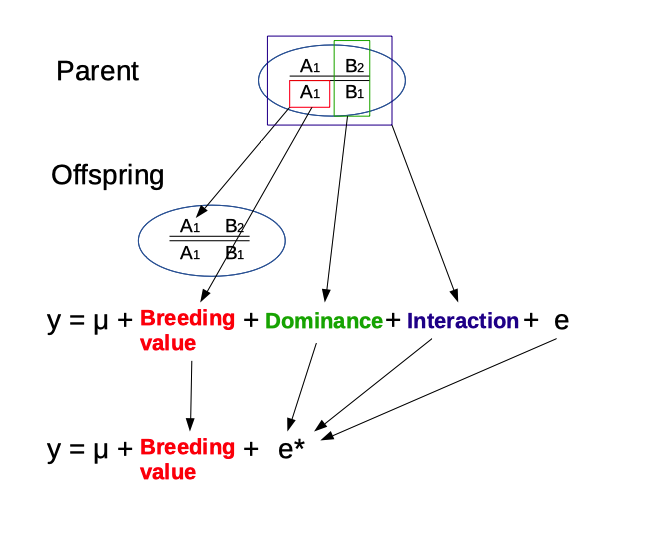
\includegraphics[width=9.26in]{odg/basicmodelrearrterm} \caption{Re-arrangment of Terms Representing Genetic Effects}\label{fig:basicmodelrearrterm}
\end{figure}
  
Equation \\eqref{eq:breedvalpredmodifiedmodel} constitutes the linear model that forms the basis for most problems of breeding value prediction in livestock breeding. Usually it is assumed that the phenotypic observations $y_{ij}$ follow a multivariate normal distribution. We have already seen in section \\ref{genetic-models} that the additive genetic effect ($a_i$) is thought to be the sum of a large number of unlinked loci that all contribute a very small amount to the total breeding value. Then by the central limit theorem it follows that $a_i$ converges to a normal distribution. By the same reasoning that the environmental effect $e_{ij}^*$ is composed of very many small contributions, also $e_{ij}^*$ converges to a normal distribution. From distribution theory it is known that the sum of two normally distributed random variables (like $a_i$ and $e_{ij}^*$) plus a fixed term (like $\mu$) is again a random variable that follows a normal distribution. We can conclude that the assumption that all the random effects ($y_{ij}$, $a_i$ and $e_{ij}^*$) in model \\eqref{eq:breedvalpredmodifiedmodel} is consistent with distribution theory. Furthermore the central limit theorem implies that in principle the number of breeding values from single loci tends to infinity. That means the total breeding value $a_i$ corresponds to a sum of infinitely many contributions. Based on the fact that in theory $a_i$ is composed of an infinite number of infinitely small components, the model in \\eqref{eq:breedvalpredmodifiedmodel} is called the __infinitesimal model__. 

Concerning the variances, it is assumed that $Var(y_{ij})$, $Var(a_i)$ and $Var(e_{ij})$ are all known. Covariances ($Cov(a_i, e_{ij})$) between genetic and environmental effects and covariances ($Cov(e_{ij}^*, e_{kl}^*)$) between environmental effects of mates $i$ and $k$ are assumed to be zero, respectively. 

Also $\mu_i$ which is used to represent the mean performance of animals in the same identifiable environment such as herd or management group or have the same sex or age, is assumed to be known.


### Decomposition of Breeding Value
As already mentioned earlier, the breeding value $a_i$ of an individual $i$ represents the average additive genetic effect that animal $i$ receives from its parents $s$ and $d$. Hence $a_i$ can be decomposed into 

\begin{equation}
a_i = {1\over 2} a_s + {1\over 2} a_d + m_i
\label{eq:breedingvalueanimalparent}
\end{equation}

where $a_s$ and $a_d$ correspond to the breeding values of parents $s$ and $d$, respectively and $m_i$ is the deviation of $a_i$ from the average breeding values of the parents and is called __Mendelian sampling__. The term $m_i$ is necessary, because two fullsibs $i$ and $k$ both having parents $s$ and $d$ receive different random samples of the set of parental alleles. Hence the breeding values $a_i$ and $a_k$ of fullsibs $i$ and $k$ are not going to be the same. The difference between breeding values $a_i$ and $a_k$ is reflected in the different Mendelian sampling terms $m_i$ and $m_k$ for fullsibs $i$ and $k$. 


## Basic Principle of Predicting Breeding Values {#principle-predic-breedingvalue}
The prediction of breeding values mostly follows the same principles. From the point of view of statistics, estimations or predictions are always a function of the observed data. When looking at the model in \\eqref{eq:breedvalpredmodifiedmodel}, we can probably guess that the observed phenotypic records ($y_{ij}$) must be corrected somehow for the identifiable environmental effects represented by $\mu_i$. The second influence that we want to consider when predicting breeding values is how "closely related" the observed record $y_{ij}$ is to the breeding value. For traits where the influence of the genetic component is not very strong, it is probably a good idea to down-weigh the information from $y_{ij}$. 

The two principles just described can be generalized as follows. Breeding values are predicted according to the following two steps. 

1. Observations are corrected for the mean performance values of animals under the same environmental conditions. The conditions are described by the effects captured in $\mu_i$. 
2. The corrected observations are weighted by a factor that reflects the amount of information that is available for the prediction of an animals breeding value.

In what follows, we have a look at how breeding values are predicted from different sources of information.



## Animal's Own Performance {#own-performance}
### Single Record {#single-record}
When one phenotypic observation per animal is the only information we have available, the predictor $\hat{a_i}$ of the breeding value $a_i$ of animal $i$ can be derived according to the following line of argument. Let us assume for a moment that we know the true breeding value $a_i$ for a population of animals. In addition to that each animal $i$ has one observation $y_i$ available. Then we plot the values of $a_i$ against the values of $y_i$ for the complete population. 

\begin{figure}
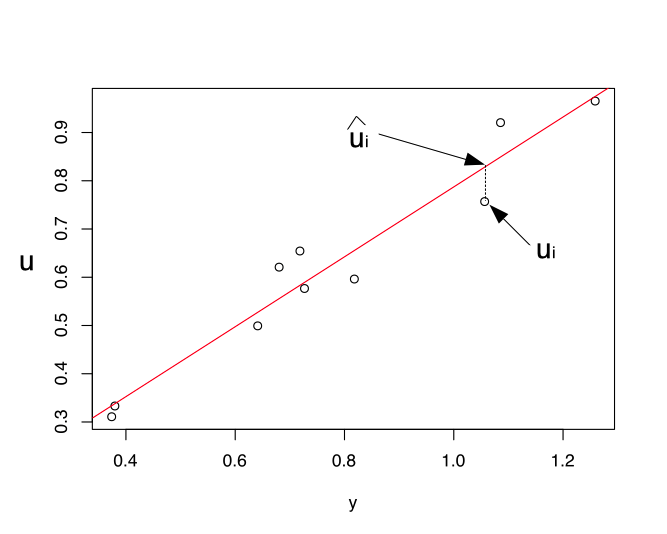
\includegraphics[width=9.26in]{odg/regbreedingvaluesinglerecord} \caption{Regression of Breeding Values onto Phenotypic Observations}\label{fig:regbreedingvaluesinglerecord}
\end{figure}

The plot in Figure \\ref{fig:regbreedingvaluesinglerecord} suggests that we fit a regression of the breeding values onto the phenotypic records. The fitted regression is represented by the red line. Hence as soon as we can draw the regression line, we can predict breeding values based on the phenotypic observations. The predicted breeding value $\hat{a_i}$ for a given $y_i$ corresponds to the value on the red line corresponding to the value of $y_i$. The slope of the regression line corresponds to the regression coefficient $b$. From regression theory, the coefficient $b$ is computed as 

\begin{align}
b &= \frac{Cov(a,y)}{Var(y)} \notag \\
  &= \frac{Cov(a,\mu + a + e)}{Var(y)}  \notag \\
  &= \frac{Cov(a,a)}{Var(y)}  \notag \\
  &= \frac{Var(a)}{Var(y)}  \notag \\
  &= h^2
\label{eq:regcoeffaony}
\end{align}

where $h^2$ corresponds to the ratio between the genetic additive and the phenotypic variance and is called __heritability__. We are using the regression coefficient to predict the breeding value for animal $i$ based on a single record $y_i$. 

\begin{align}
\hat{a_i} &= b * (y_i - \mu) \notag \\
          &= h^2 * (y_i - \mu)
\label{eq:predbreedvalueownsinglerecord}
\end{align}

From that it follows that the predicted breeding value for an animal based on a single own performance record corresponds to the observation corrected for the general mean $\mu$ times the heritability. The correlation between the selection criterion, in our case the phenotypic record and the true breeding value is known as the accuracy of the prediction. It provides a means of evaluating the different selection criteria. The higher the correlation between selection criterion and breeding value, the better is the prediction. Sometimes the accuracy of evaluation is reported in terms of reliability ($r^2$) which corresponds to the squared correlation between selection criterion and true breeding value. With a single own performance record per animal, the correlation is 

\begin{align}
r_{a,y} &= \frac{Cov(a, y)}{\sigma_u \ \sigma_y} \notag \\
        &= \frac{\sigma_u^2}{\sigma_u \ \sigma_y} \notag \\
        &= \frac{\sigma_u}{\sigma_y} \notag \\
        &= h
\label{eq:corownperftruebreedingvalue}
\end{align}

An alternative way to assess the quality of the breeding value prediction is to compute the variance of the predicted breeding values. 

\begin{align}
Var(\hat{a_i}) &= Var(by) = Var(h^2y) \notag \\
               &= h^4 Var(y) \notag \\
               &= r_{a,y}^2 h^2 \sigma_y^2 \notag \\
               &= r_{a,y}^2 \sigma_a^2
\label{eq:varpredictedbreedingvalue}
\end{align}

Hence the variance of the predicted breeding values corresponds to the product of the reliability times the genetic additive variance. The expected response ($R$) to selection on the basis of one record per animal is 

\begin{equation}
R = i * r_{a,y}^2 * \sigma_y = i * h^2 * \sigma_y
\label{eq:selectionresponseownperformance}
\end{equation}

where $i$, the selection intensity refers to the superiority of selected individuals above population mean expressed in phenotypic standard deviation.


### Repeated Records {#repeatedrecords}
When animals get older, it is likely that we can observe multiple measurements for the same trait. An example is milk yield in dairy cows where a cow might have repeated lactation records. The breeding value of an animal may be predicted based on the mean of the repeated records. With repeated records, an additional resemblance between the records of an animal due to permanent environmental factors occurs. The between-animal variance is partly genetic and partly caused by permanent environmental effects. The within-animal variance is attributed to differences between the successive measurements of the animal arising from temporary environmental variations, i.e., from environmental factors that change over time. The variance of observations ($Var(y)$) can therefore be partitioned as 

\begin{equation}
Var(y) = Var(a) + Var(pe) + Var(te)
\label{eq:varrepeatedrecords}
\end{equation}

where $Var(a)$ is the genetic additive variance, $Var(pe)$ the variance due to permanent environmental effects and $Var(te)$ the variance due to temporary environmental effects. 

The intra-class correlation $t$ is defined as the ratio of the genetic plus the permanent environmental variance divided by the phenotypic variance.

\begin{equation}
t = \frac{Var(a) + Var(pe)}{Var(y)}
\label{eq:intraclasscorrelation}
\end{equation}

The term $t$ is also called __repeatability__ and it measures the correlation between the records of an individual. From \\eqref{eq:intraclasscorrelation} it follows that 

\begin{equation}
1-t = \frac{Var(te)}{Var(y)}
\label{eq:oneminusintraclasscorrelation}
\end{equation}

With this model, it is assumed that the repeated records on the animal are the same trait. Therefore the genetic correlation between all pairs of records is one. We also assume that all records have equal variance and that the environmental correlations between all pairs of records are equal. Let $\tilde{y}$ represent the mean of $n$ records on animal $i$ which means

\begin{align}
\tilde{y_i} &= {1\over n} \sum_{k=1}^n y_{ik} \notag \\
            &= {1\over n} \sum_{k=1}^n ( \mu + a_i + pe_i + te_{ik}) \notag \\
            &= \mu + a_i + pe_i + \sum_{k=1}^n te_{ik}
\label{eq:meanrepeatedrecords}
\end{align}

In this case, we use the mean ($\tilde{y_i}$) to predict the breeding value ($\hat{a_i}$)

\begin{equation}
\hat{a_i} = b(\tilde{y_i} - \mu)
\label{eq:predbreedingvaluerepeatedrecords}
\end{equation}

where 

\begin{equation}
b = \frac{Cov(a,\tilde{y})}{Var(\tilde{y})}
\label{eq:regcoeffrepeatedrecords}
\end{equation}

The single elements are computed as

\begin{equation}
Cov(a,\tilde{y}) = Cov(a, \mu + a + pe + {1\over n} \sum_{k=1}^n te_k) = Var(a) = \sigma_u^2
\label{eq:covayrepeatedrecords}
\end{equation}

and 

\begin{equation}
Var(\tilde{y}) = Var(a) + Var(pe) + {1\over n} Var(te)
\label{eq:varyrepeatedrecords}
\end{equation}

Expressing \\eqref{eq:varyrepeatedrecords} in terms of \\eqref{eq:intraclasscorrelation} and \\eqref{eq:oneminusintraclasscorrelation} leads to 

\begin{align}
Var(\tilde{y}) &= t * \sigma_y^2 + {1\over n} (1-t) * \sigma_y^2 \notag \\
               &= {1\over n}\left( n*t + (1-t) \right) \sigma_y^2 \notag \\
               &= \frac{1 + (n-1)t}{n} \sigma_y^2
\label{eq:varyastrepeatedrecords}
\end{align}

Inserting this into \\eqref{eq:regcoeffrepeatedrecords} results in 

\begin{align}
b &= \frac{Cov(a,\tilde{y})}{Var(\tilde{y})} \notag \\
  &= \frac{n \sigma_u^2}{(1 + (n-1)t) \sigma_y^2} \notag \\
  &= \frac{nh^2}{1 + (n-1)t}
\label{eq:regcoeffrepeatedrecordsresult}
\end{align}

When we predict the breeding value $a_i$ of animal $i$ using repeated records, the regression coefficient $b$ depends on 

1. the heritability ($h^2$) 
2. the repeatability ($t$) and 
3. the number ($n$) of repeated records per animal


The difference between repeated records of an animal is assumed to be due to temporary environmental differences between successive performances. However, if successive records are known to be affected by factors which influence performance, these must be corrected for. For instance, differences in age at calving in first and second lactations may influence milk yield in first and second lactation. Such age differences should be adjusted for before using the means of both lactations for breeding value prediction.

The accuracies of the predicted breeding value using repeated records is 

\begin{align}
r_{a,\tilde{y}} &= \frac{Cov(a,\tilde{y}) }{\sigma_u \sigma_y} \notag \\
                &= \frac{\sigma_u^2}{\sigma_u \sqrt{(1 + (n-1)t)/n \sigma_y^2}} \notag \\
                &= h \sqrt{n/(1 + (n-1)t)} \notag \\
                &= \sqrt{nh^2/(1 + (n-1)t)} \notag \\
                &= \sqrt{b}
\label{eq:accrepeatedrecords}
\end{align}

The expected response to selection using repeated records will be covered in an exercise.


## Progeny Records {#progenyrecords}
For traits that are recorded only on female animals, the prediction of breeding values for male animals (sires) is usually based on the mean of their female progeny. This is typical in dairy cattle, where bulls are evaluated on the basis of their daughters. Let $\bar{y_i}$ be the mean of single records of $n$ daughters of sire $i$ with the assumption that the daughters are only related through the sire (paternal half-sibs), the predicted breeding value of sire i can then be computed as 

\begin{equation}
\hat{a_i} = b * (\bar{y_i} - \mu)
\label{eq:predictedbreedingvalueprogeny}
\end{equation}

where 

\begin{equation}
b = \frac{Cov(a, \bar{y})}{Var(\bar{y})}
\label{eq:regressioncoefficientprogeny}
\end{equation}

and 

\begin{align}
\bar{y} &= {1 \over n} \sum_{k=1}^n y_k \notag \\
        &= {1 \over n} \sum_{k=1}^n (\mu + a_k + e_k) \notag \\
        &= \mu + {1 \over n} \sum_{k=1}^n (a_k + e_k) \notag \\
        &= \mu + {1 \over n} \sum_{k=1}^n (1/2 a_s + 1/2 a_{dk} + m_k + e_k) \notag \\
        &= \mu + 1/2 a_s + {1 \over n} \sum_{k=1}^n (1/2 a_{dk} + m_k + e_k) \notag \\
        &= \mu + 1/2 a_s + {1 \over n} \sum_{k=1}^n 1/2 a_{dk} + {1 \over n} \sum_{k=1}^n e_k
\end{align}


In the current case of using progeny records to predict a breeding value, we have 

\begin{align}
Cov(a, \bar{y}) &= Cov(a, {1\over 2}a_s + {1\over 2}{1\over n}\sum_{k=1}^n a_{d,k} + {1\over n}\sum_{k=1}^n m_k + {1\over n}\sum_{k=1}^n e_k) \notag \\
                &= Cov(a, {1\over 2}a_s) \notag \\
                &= {1\over 2} Cov(a, a_s) \notag \\
                &= {1\over 2} \sigma_u^2
\end{align}

where $a_s$ and $a_{d,k}$ denote the breeding values of sire $s$ and dam $d$ of offspring $k$, respectively and $m_k$ and $e_k$ stand for the mendelian sampling and the environmental effect of daughter $k$. Using the same principles as in section \\ref{repeatedrecords}, we get

\begin{equation}
Var(\bar{y}) = (t + (1-t)/n) \sigma_y^2
\label{eq:variancedaughtermean}
\end{equation}

where $\sigma_y^2 = Var(a) + Var(e) = \sigma_u^2 + \sigma_e^2$.

Assuming there is no environmental covariance between half-sib records and the intra-class correlation $t$ is $\frac{1/4 \sigma_u^2}{\sigma_y^2}$. Then we can compute the regression coefficient as 

<!-- ---------------------------------------------------- --
  -- TODO: Explain how $Var(\bar{y})$ is derived          --
  --                                                      --
  -- ---------------------------------------------------- -->

\begin{align}
b &= \frac{1/2 \sigma_u^2}{(t + (1-t)/n) \sigma_y^2} \notag \\
  &= \frac{1/2 h^2 \sigma_y^2}{({1\over 4}h^2 + (1 - {1\over 4}h^2)/n) \sigma_y^2} \notag \\
  &= \frac{2nh^2}{nh^2 + (4-h^2)} \notag \\
  &= \frac{2n}{n + (4-h^2)/h^2} \notag \\
  &= \frac{2n}{n+k}
\label{eq:regcoeffprogeny}
\end{align}

with $k=\frac{4-h^2}{h^2}$. 

The term $k$ is constant for any assumed heritability ($h^2$). The regression coefficient ($b$) depends on the heritability and number of progeny and converges towards a limit of $2$ as the number of daughters increases.

The accuracy of the estimated breeding value is

\begin{align}
r_{a, \bar{y}} &= \frac{Cov(a, \bar{y})}{\sqrt{Var(a) Var(\bar{y})}} \notag \\
               &= \frac{1/2 h^2 \sigma_y^2}{\sqrt{h^2 \sigma_y^2 ({1\over 4}h^2 + (1 - {1\over 4}h^2)/n) \sigma_y^2}} \notag \\
               &= \frac{1/2 h}{\sqrt{{1\over 4}h^2 + (1 - {1\over 4}h^2)/n}} \notag \\
               &= \sqrt{\frac{nh^2}{nh^2 + (4-h^2)}} \notag \\
               &= \sqrt{\frac{n}{n + k}}
\label{eq:accuracyprogeny}
\end{align}

The term for $r_{a, \bar{y}}$ in \\eqref{eq:accuracyprogeny} approaches $1$ as the number of progeny increases, assuming $k$ is constant. The reliability ($r_{a, \bar{y}}^2$) of the predicted breeding value is $n/(n+k)$ and corresponds to $1/2 * b$ computed in \\eqref{eq:regcoeffprogeny}. 


\end{comment}

  \bibliography{qg2021.bib}

\end{document}
